\section{Results}\label{sec:results}

\noindent\textbf{Main findings at a glance.}
\begin{itemize}
  \item \emph{Small data:} on one month the clusters are 4--6$\times$ slower than a
        single Python process, because start-up costs 13--23\,s per job.
  \item \emph{Large data:} on two years four workers are up to 4.0$\times$ faster than
        one; Spark DataFrame is the fastest engine, up to 5.1$\times$ faster than serial.
  \item \emph{Single host vs.\ cloud:} two Azure VMs scale more regularly than two
        containers on one host, but each VM is slower.
\end{itemize}

\subsection{Method}
For each cluster size $N\in\{1,2,3,4\}$ the cluster is rebuilt from scratch, a data
tier is loaded into HDFS, and every combination of job and engine is run three times
(twice on tier XL) by \texttt{scripts/run\_benchmark.sh}; the serial baseline runs
once per tier in a single process. Runs of one configuration follow each other, so
repetitions 2 and 3 start with a warm operating-system cache. We report the mean
wall-clock time from job submission to completion, which includes start-up and
scheduling overhead, and its standard deviation. In total we recorded 561 runs on the
local cluster and 225 on Azure, all successful. With $T_1$ the time of the same engine
on one worker and $T_\text{serial}$ the time of the single-process baseline, we use
\begin{equation}
S_\text{rel}(N)=\frac{T_1}{T_N},\qquad E(N)=\frac{S_\text{rel}(N)}{N},\qquad
S_\text{abs}(N)=\frac{T_\text{serial}}{T_N}.
\end{equation}
To estimate the non-parallel fraction we use the Karp--Flatt
metric~\cite{karp1990measuring}, $e=\frac{1/S_\text{rel}-1/N}{1-1/N}$, and interpret
it with Amdahl's law~\cite{amdahl1967validity}. For weak scaling, each worker receives
three months of data (tiers W3, M, W9, L for $N=1..4$) and the efficiency is
$T(1,\text{W3})/T(N,3N\text{ months})$.

\subsection{Analytics output}
\Cref{fig:run} shows one real run: the \texttt{routes} job on tier L with four
workers. Hadoop splits the 24 monthly blocks into 24 map tasks, 20 of them on the
worker that stores the block; the combiner shrinks 39.7~million map outputs to
\num{537298} records before the shuffle, and the job writes \num{50127} routes in
60.8\,s. \Cref{fig:analytics} shows the answers to the three questions for the full year 2024
(tier L, \num{39705145} valid trips). Demand peaks at 18:00 with 2.82~million trips
over the year and is lowest at 04:00 (0.23~million); the busiest zone--hour pair is
Midtown Center at 18:00 (\num{164630} pickups). The busiest zones differ in
\emph{when} they are busy: Midtown peaks in the evening rush hour, the Upper East Side
during the day, and JFK Airport is the only one with substantial traffic after
midnight. The five most frequent routes all start and end in the Upper East Side or
Midtown, i.e.\ short trips inside Manhattan. Average fares grow with distance, while
the credit-card tip rate falls from 28.8\% of the fare for trips under one mile to
17.1\% for trips over 20~miles.

\begin{figure}[t]
\begin{lstlisting}[style=terminal]
$ docker exec master /opt/scripts/run_job.sh mr routes L 4
INFO mapreduce.JobSubmitter: number of splits:24
INFO impl.YarnClientImpl: Submitted application
     application_1795551341851_0087
INFO mapreduce.Job:  map 0% reduce 0%
INFO mapreduce.Job:  map 50% reduce 0%
INFO mapreduce.Job:  map 100% reduce 45%
INFO mapreduce.Job:  map 100% reduce 100%
INFO mapreduce.Job: Job job_1795551341851_0087 completed
     successfully
  Launched map tasks=24       Data-local map tasks=20
  Map input records=41169720
  Map output records=39705145
  Combine output records=537298
  Reduce shuffle bytes=6656616
  Reduce output records=50127
SECONDS 60.84
$ sort -k2 -nr outputs/mr-routes-L.tsv | head -3
237|236    275994
236|237    237909
237|237    184456
\end{lstlisting}
\caption{A real run (abridged; timestamps removed): \texttt{routes} on tier L with
four workers, Hadoop progress and job counters, the run time printed by
\texttt{run\_job.sh}, and the three most frequent routes in the output
(zone 237 = Upper East Side South, 236 = Upper East Side North).}\label{fig:run}
\end{figure}

\begin{figure*}[t]
\centering
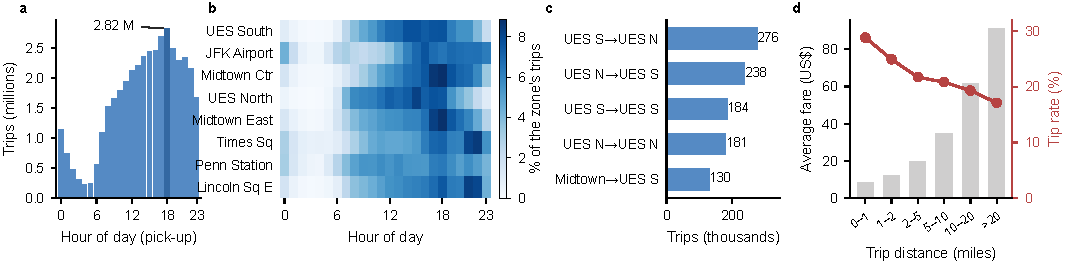
\includegraphics[width=\textwidth]{figures/analytics_L.pdf}
\caption{What the three jobs found in the 39.7~million valid trips of 2024 (tier L,
identical for all engines). (a)~\texttt{demand}: trips per hour of day, peak at 18:00.
(b)~\texttt{demand}: hourly profile of the eight busiest pick-up zones, each row
normalised to the zone's total (UES = Upper East Side). (c)~\texttt{routes}: the five
most frequent pick-up$\rightarrow$drop-off zone pairs. (d)~\texttt{fare}: average fare
(bars) and credit-card tip rate (line) per distance band.}\label{fig:analytics}
\end{figure*}

\subsection{Run time and speedup on the local cluster}
\Cref{fig:scaling} shows the \texttt{routes} job on every tier; the other two jobs
behave in the same way, and \cref{tab:summary} lists all jobs for tier L.

\begin{figure*}[t]
\centering
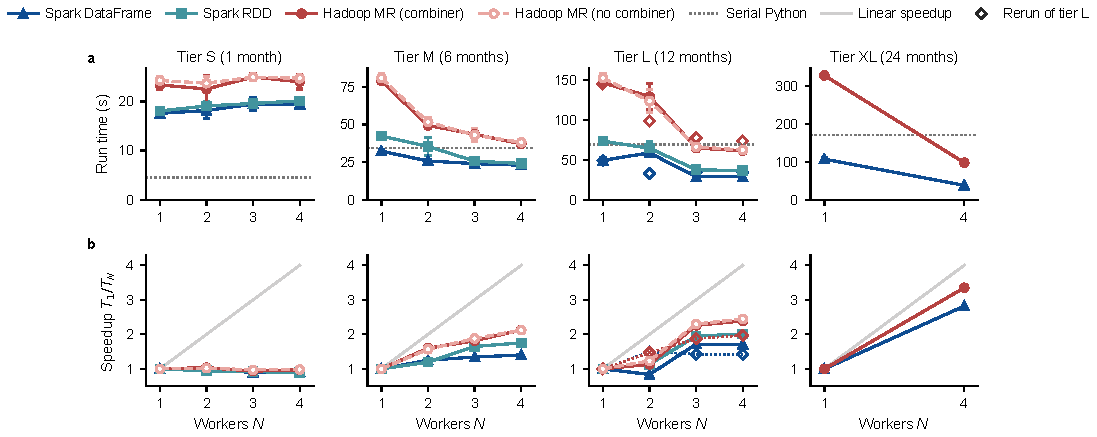
\includegraphics[width=\textwidth]{figures/scaling_routes.pdf}
\caption{Strong scaling of the \texttt{routes} job on the local cluster, one column per
data tier. (a)~Mean run time with one standard deviation; dotted: serial baseline.
(b)~Relative speedup $T_1/T_N$; grey: linear speedup. Open diamonds: the warm runs of
the later cache experiment on tier L (\cref{tab:cache}), which do not show the dip at
$N=2$. Tier XL was run with 1 and 4 workers only.}\label{fig:scaling}
\end{figure*}

\begin{table*}[t]
\centering
\caption{Tier L (12 months, 1.93\,GiB) on the local cluster: mean run time (s) per
number of workers, and relative speedup, efficiency, speedup over the serial baseline
and Karp--Flatt serial fraction at $N=4$. Bold: fastest engine of each job. Standard
deviations are in
\texttt{results/summary.csv}.}\label{tab:summary}
\begin{tabular*}{\textwidth}{@{\extracolsep{\fill}}llrrrrrrrr@{}}
\toprule
Job & Engine & $T_1$ & $T_2$ & $T_3$ & $T_4$ & $S_\text{rel}(4)$ & $E(4)$ & $S_\text{abs}(4)$ & $e(4)$ \\
\midrule
\inputrows{generated/summary_table.tex}
\bottomrule
\end{tabular*}
\end{table*}

\textbf{Small data (tier S).} The serial baseline needs 4.3--4.5\,s per job, whereas
every cluster configuration needs 17--23\,s with Spark and 22--27\,s with MapReduce,
independently of $N$ ($S_\text{rel}\approx1$). The run time is almost entirely fixed
cost: submitting the application, starting the YARN application master and the
executor or task JVMs, and writing the output.

\textbf{Medium and large data.} From tier M on, adding workers reduces the run time.
At $N=4$, MapReduce reaches $S_\text{rel}=2.0$--$2.2$ on tier M and 2.4--2.8 on tier
L; Spark RDD 1.7--1.8 and 2.0--2.4; Spark DataFrame 1.4--1.6 and 1.7--1.9. On tier XL,
MapReduce speeds up by 3.35--3.97 from one to four workers ($E=0.84$--$0.99$) and the
DataFrame engine by 2.25--3.05. In absolute terms Spark DataFrame is always fastest:
on tier L with four workers it needs 29\,s per job, 2.2--2.4$\times$ faster than the
serial baseline, and on tier XL 38--39\,s, 3.6--5.1$\times$ faster than the serial
baseline (139--195\,s). On tier L, Hadoop MapReduce on one worker is 2.1--2.6$\times$
slower than the serial baseline and only matches it with three or four workers on tier L
($S_\text{abs}(4)=1.03$--$1.13$); on tier XL it is 1.4--1.75$\times$ faster.

\textbf{The two-worker anomaly.} On tier L the step from one to two workers gives
almost no gain (MapReduce $S_\text{rel}(2)=1.08$--$1.34$; Spark DataFrame 0.84--1.18,
i.e.\ \texttt{routes} became slower), MapReduce run times at $N=2$ vary strongly
(standard deviation up to 23\,s), and the step from two to three workers is then
\emph{superlinear} (MapReduce 1.8--2.1$\times$ for 1.5$\times$ the workers). The same
step on tier M is regular ($S_\text{rel}(2)=1.5$--$1.6$ for MapReduce). A controlled
rerun did not reproduce the anomaly (\cref{sec:discussion}).

\textbf{Weak scaling.} With three months of data per worker
(\cref{fig:weak}) the efficiency at four workers is 0.79 for Spark DataFrame, 0.75 for
Spark RDD and 0.70 (0.67 without combiner) for MapReduce, averaged over the three jobs.

\begin{figure}[t]
\centering
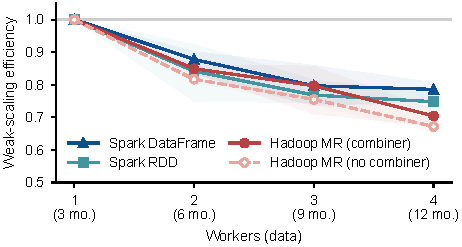
\includegraphics[width=\columnwidth]{figures/weak_scaling.pdf}
\caption{Weak-scaling efficiency $T(1,\text{W3})/T(N,3N\text{ months})$ with three
months of data per worker: mean of the three jobs (lines) and their range
(shading).}\label{fig:weak}
\end{figure}

\subsection{Effect of the combiner}
\Cref{fig:combcloud}a shows the data shuffled from map to reduce tasks on tier L,
from the MapReduce job counters. All three jobs emit the same 39.7~million map output
records; the combiner shrinks the shuffle by a factor of 72 for \texttt{routes}, 309
for \texttt{demand} and about \num{100000} for \texttt{fare}, where the records
collapse to 216 per run (1.1\,GiB to 12\,KiB). The run-time effect depends on the
job: on one worker \texttt{fare} is 24\% faster with the combiner (169 vs.\ 223\,s)
and 20\% faster at $N=4$, whereas \texttt{demand} and \texttt{routes} change by less
than the run-to-run variation (\cref{tab:summary}). On Azure with two workers the
combiner saves 29\% for \texttt{fare} (236 vs.\ 332\,s) and 7--10\% for the other jobs.

\begin{figure}[t]
\centering
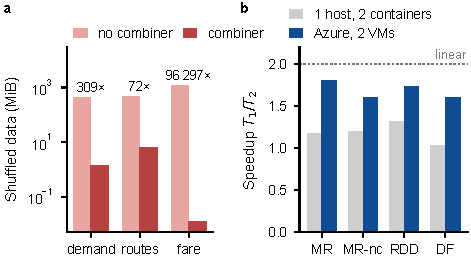
\includegraphics[width=\columnwidth]{figures/combiner_cloud.pdf}
\caption{(a)~Data shuffled per MapReduce job on tier L without and with the combiner
(log scale; labels: reduction factor). (b)~Speedup from one to two workers on tier L,
run times summed over the three jobs: two containers on one host vs.\ two Azure VMs
(MR-nc: MapReduce without combiner).}\label{fig:combcloud}
\end{figure}

\subsection{Public cloud}
\Cref{fig:combcloud}b compares the same software and configuration on the local
containers and on the Azure VMs. On one worker, Azure is 2.0$\times$ slower for the
serial baseline (388 vs.\ 197\,s for the three jobs) and 2.5--3.3$\times$ slower for
the cluster engines (e.g.\ Spark DataFrame 449 vs.\ 154\,s, MapReduce 1221 vs.\
463\,s). On the other hand the Azure cluster scales better from one to two workers:
on tier L the summed speedup is 1.60--1.80 on Azure (efficiency 0.80--0.90) against
1.03--1.31 locally. On tier M both environments behave similarly (Azure MapReduce
1.68--2.03, Spark 1.37--1.65; local MapReduce 1.52--1.64, Spark 1.19--1.40). On tier S
the cloud cluster shows no speedup either ($S_\text{rel}=0.97$--$1.12$), with a fixed
cost of about 40\,s per job for Spark and 55\,s for MapReduce.

\subsection{Correctness}
For every tier and cluster size, the outputs of Hadoop MapReduce (with and without
combiner), Spark RDD and Spark DataFrame agree with the serial baseline
(\texttt{compare\_outputs.py}; money sums agree to within the 0.01 rounding of the
printed values). The outputs computed on Azure are identical to the local ones.
